n Submissions to examination are made using [e-mail/Blackboard] to Ella KolkowskaDeadline 2021-05-28 at 1 p.mPlagiari%Created by, Mikael Andersson and the whole Network engineering class of 2019 (MDH)
%edited by Johannes Henriksson

% Title
\title{Latex Mall [ORU] v4.2}

% Document type
\documentclass[11pt, titlepage, a4paper]{article}

% Preamble

% ==================== Packages ====================
% Character Encoding
\usepackage[T1]{fontenc}
\usepackage[utf8]{inputenc}
\usepackage{lmodern}
\usepackage{xcolor}
\usepackage[english]{babel} % <-- Change language used here. Rememeber to clean all the aux files before building document.
\usepackage{csquotes}
\usepackage{microtype}

% Bibliography & References Formatting
\usepackage[style=apa6,backend=biber,dateabbrev=false]{biblatex}
\DeclareLanguageMapping{english}{english-apa}

% Appendices Formatting
\usepackage[titletoc,title]{appendix}
%\renewcommand\appendixtocname{Bilagor}     % <-- If needed to manually change appendice names
%\renewcommand\appendixpagename{Bilagor}    % <-- If needed to manually change appendice names

% Text Formatting
\usepackage{marginnote}
\usepackage[absolute]{textpos}
\usepackage[normalem]{ulem}
\sloppy
\usepackage{subcaption}





% Document Formatting
\usepackage{fancyhdr}
\usepackage{enumerate}
\usepackage{enumitem}
\usepackage{listings}
%\renewcommand{\lstlistlistingname}{Listor}   % If needed to manually change list of lists's name in ToC.
%\renewcommand{\lstlistingname}{Lista}        % If needed to manually change list's name in document.
\usepackage[a4paper,hmargin=1in,vmargin=3cm]{geometry}
\usepackage[section]{placeins}
\setcounter{tocdepth}{5}
\setcounter{secnumdepth}{5}
\usepackage{titlesec}
\titleformat{\paragraph}
{\normalfont\normalsize\bfseries}{\theparagraph}{1em}{}
%\titlespacing*{\paragraph}{0pt}{3.25ex plus 1ex minus .2ex}{1.5ex plus .2ex}


% List code style
\lstset{
    backgroundcolor=\color[rgb]{0.92,0.92,0.92},
    basicstyle=\ttfamily,
    columns=fullflexible,
    keepspaces=true,
    frame=single,
    showspaces=false,
    showstringspaces=false,
    showtabs=false,
    tabsize=2,
    captionpos=b,
    breaklines=true,
    postbreak=\mbox{\textcolor{red}{$\hookrightarrow$}\space},
    keywordstyle=\color[rgb]{0,0,1},
    commentstyle=\color[rgb]{0.133,0.545,0.133}
}

% Urls & Hyperref
\usepackage{url}
\usepackage[pdfborder={0 0 0}, colorlinks=true, urlcolor=blue, citecolor=red, bookmarks=trufalse]{hyperref}

% Image and Table Formatting
\usepackage{tabularx}
\usepackage{caption}
\usepackage{graphicx}
\usepackage{array}
\usepackage{diagbox}
\usepackage{chngcntr}
\usepackage{multirow}
\usepackage{color, colortbl}

% Tikz
\usepackage{tikz}
\usepackage{pgfplots}

\usepackage{float}

% Math
\usepackage{amsmath}
\usepackage{amsfonts}
\usepackage{mathtools}
\usepackage{bm}

% Other
\usepackage{lipsum}
%\setlength\parindent{0pt}

% Abbreviations
\usepackage{longtable}
\usepackage[acronym,toc]{glossaries}

% Other
\usepackage{lipsum}
%\setlength\parindent{0.5in}
\usepackage{dirtytalk}
\pgfplotsset{compat=1.17}



\usepackage{rotating}

\bibliography{static/biblio}

%============================== Custom macros for document

%=============== Front page info
%% Logo info
\def\tLogoLocation{static/pics/logoKransColorENG.png}
\def\tLogoWidth{15mm}

%% School info
\def\tSchoolName{University NAME}
\def\tAcademyName{DEPAETMENT}
\def\tSchoolLocation{City}


%% Course info
% Leave the fields for titles, authors and teachers blank if you don't need them.
% e.g. \tTitleThree{}
% They will automatically be hidden on the front page.

\def\tCourseName{COURSE NAME}
\def\tTitleOne{TITLE} % the title should explain as much as possible what the report is about, but, be as short as possible
\def\tTitleTwo{} % <-- Set to {} to hide
\def\tTitleThree{}   % <-- Set to {} to hide


%% Author info
\def\tAuthorTitle{Authors:}     % <-- Set to {} to hide

\def\tAuthorOneName{STUDENT 1}       % <-- Set to {} to hide
\def\tAuthorOneEmail{}
%======
\def\tAuthorTwoName{STUDENT 2}       % <-- Set to {} to hide
\def\tAuthorTwoEmail{}
%======
\def\tAuthorThreeName{}     % <-- Set to {} to hide
\def\tAuthorThreeEmail{}
%======
\def\tAuthorFourName{}    % <-- Set to {} to hide
\def\tAuthorFourEmail{}

%% Teacher info
\def\tTeacherOneTitleAndName{Examiner: NAME NAME}
\def\tTeacherOneEmail{EMAIL}
\def\tTeacherOneLocation{\tSchoolName, \tSchoolLocation}
%======
\def\tTeacherTwoTitleAndName{Supervisor: NAME NAME}  % <-- Set to {} to hide
\def\tTeacherTwoEmail{EMAIL}
\def\tTeacherTwoLocation{\tSchoolName, \tSchoolLocation}

\def\tTeacherThreeTitleAndName{Supervisor: NAME NAME}  % <-- Set to {} to hide
\def\tTeacherThreeEmail{EMAIL}
\def\tTeacherThreeLocation{\tSchoolName, \tSchoolLocation}

%% Misc
\def\tDate{\today}      % Use \today or set a date manually

%=============== Document Headers
\def\mLHeader{\tAuthorOneName, \tAuthorTwoName}
\def\mRHeader{Doc Header}
%============================== End of macros

%============== PDF metadata
\def\tKeyWords{Some keywords here}%just make the bracket empty if no keywords are needed

\hypersetup{
pdftitle={\tTitleOne},
pdfauthor={\mLHeader},
pdfkeywords={\tKeyWords},
pdfsubject={\mRHeader}
}
%==========================


%
\newcommand\subsubsubsection{\@startsection{paragraph}{4}{\z@}{-2.5ex\@plus -1ex \@minus -.25ex}{1.25ex \@plus .25ex}{\normalfont\normalsize\bfseries}}
\newcommand\subsubsubsubsection{\@startsection{subparagraph}{5}{\z@}{-2.5ex\@plus -1ex \@minus -.25ex}{1.25ex \@plus .25ex}{\normalfont\normalsize\bfseries}}


% Page style
\pagestyle{fancy}
\marginparsep = 10pt
\renewcommand*{\marginfont}{\footnotesize}

% Table of Contents
\renewcommand\contentsname{Table of Contents}
\addto\captionsenglish{% Replace "english" with the language you use
  \renewcommand{\contentsname}%
    {Table of Contents}%
}
\newcommand{\HRule}{\rule{\linewidth}{0.5mm}}
\newcommand{\circR}{\textsuperscript{\textregistered}}

\makeatother
\makeglossaries



% Document begins
\begin{document}
    \pagenumbering{gobble}
    % Title
    \begin{titlepage}
        \begin{center}
    %\begin{figure}[h]
        %\begin{center}
        %     \includegraphics[width=40mm]{\tLogoLocation}
        %\end{center}
       
    %\end{figure}

    \Large \tSchoolName \\
    \Large \tAcademyName \\
    \Large \tSchoolLocation \\

    \noindent\makebox[\linewidth]{\rule{\textwidth}{0.4pt}} \\ [0.5cm]

    \Large{\tCourseName} \\ [1.0cm]

%============================================================
% Title management

    \Huge \textbf{{\tTitleOne}} \\ [0.5cm]
    \ifx
        \tTitleTwo \empty
            %nothing
        \else
            \LARGE {\uppercase{\tTitleTwo}} \\
    \fi
    \ifx
        \tTitleThree \empty
            ~\\ [0.5cm]
        \else
            \huge \textbf{\uppercase{\tTitleThree}} \\ [1cm]
    \fi

%============================================================
% Author management

    \ifx
        \tAuthorTitle \empty
            %nothing
        \else
            \LARGE \textbf{\underline{\smash{\tAuthorTitle}}} \\ [0.2cm]
    \fi
    
    
    \LARGE \tAuthorOneName \\
    %\large \href{mailto:\tAuthorOneEmail}{\tAuthorOneEmail} \\
    
    \ifx
        \tAuthorTwoName \empty
            %nothing
        \else
            \LARGE \tAuthorTwoName \\
            %\large \href{mailto:\tAuthorTwoEmail}{\tAuthorTwoEmail} \\
    \fi
    \ifx
        \tAuthorThreeName \empty
            %nothing
        \else
            \LARGE \tAuthorThreeName \\
            %\large \href{mailto:\tAuthorThreeEmail}{\tAuthorThreeEmail} \\
    \fi
    \ifx
        \tAuthorFourName \empty
            %nothing
        \else
            \LARGE \tAuthorFourName \\
            %\large \href{mailto:\tAuthorFourEmail}{\tAuthorFourEmail} \\
    \fi

    \vspace*{\fill}

%============================================================
% Teacher management

    \begin{flushleft}
        \Large \tTeacherOneTitleAndName \\
        \begin{minipage}[t]{0,7\textwidth}
            %\large \href{mailto:\tTeacherOneEmail}{\tTeacherOneEmail} \\
            \large \tTeacherOneLocation
        \end{minipage} \\ [0.5cm]

        \ifx
            \tTeacherTwoTitleAndName \empty
                %nothing
            \else
                \Large \tTeacherTwoTitleAndName \\
                \begin{minipage}[t]{0,7\textwidth}
                    %\large \href{mailto:\tTeacherTwoEmail}{\tTeacherTwoEmail} \\
                    \large \tTeacherTwoLocation
                \end{minipage} \\ [0.5cm]
        \fi
         
        \ifx
            \tTeacherThreeTitleAndName \empty
                %nothing
             \else
                \Large \tTeacherThreeTitleAndName \\
                \begin{minipage}[t]{0,7\textwidth}
                    %\large \href{mailto:\tTeacherThreeEmail}{\tTeacherThreeEmail} \\
                    \large \tTeacherThreeLocation
                \end{minipage} \\ [0.5cm]
        \fi
    \end{flushleft}

%============================================================

    \large \tDate

\end{center}
    \end{titlepage}

    % Page style
    \pagestyle{fancy}
    \fancyhead[L]{\mLHeader}
    \fancyhead[R]{\mRHeader}
    \setlength{\headheight}{14pt}
    \fancyfoot[L]{}
    \fancyfoot[R]{}
    \renewcommand{\headrulewidth}{0.4pt}
    \renewcommand{\footrulewidth}{0.4pt}

    % Reset of counters after each section
    \counterwithin{figure}{section}
    \counterwithin{table}{section}
    \counterwithin{lstlisting}{section}

% -============================Summary=======================================
    \pagenumbering{Alph}
  \hypersetup{linkcolor=black}

  %TC:ignore
  \def\mPrintSummary{sum}    % Set to {} to skip printing summary.
  \ifx
    \mPrintSummary \empty
      % nothing
    \else
        %\pdfbookmark{\contentsname}{Abstract}
        \vspace*{\fill}
        \begin{center}
            \begin{large}
                \textbf{Abstract}
            \end{large}
        \end{center}
        %\begin{abstract}
        \textit{% This section should simply be just this: a summary of the entire report. A suitable length is about 200 - 250 words. A good rule of thumb is that summary should be kept as short as possible, it should be compact but still clear, informative and attract interest. Give the most important facts and summarize everything that is essential in the report. The following should be included:

% - Presentation / introduction of the area of work
% - A comprehensive presentation of the task including purpose and question
% - Motivation as to why the area and the task are important and interesting
% - General description of how you attacked the task, what you did
% - Summary of results and conclusions and what your work supports

% No details should be included in the summary, nor the description of how the report is structured.
% The summary should be read completely independent of the rest of the report, and by a fairly wide range of of readers (from experts to novice). It should provide a good basis for readers to judge whether they are interested in reading the entire report.
% The summary is the part of a report that is read the most and by most of the people. Therefore, it is extremely important that you write a good summary. You need to have a good grasp of the contents of the reports as you write the summary, and when the entire report is complete you should review and, if necessary, the summary should be summarized so that it corresponds to the report.






Short summery of the entire report and or document}      % Quick summary of the whole paper.
        %\end{abstract}
        
        
        \vspace*{\fill}
        \textit{Keywords:} \tKeyWords
      \newpage
  \fi
  %TC:endignore

\glsresetall % resets all abbreviations after the abstract
%========================== Table of contents =========================
  \pagenumbering{roman}  
   \hypersetup{linkcolor=black}
    %TC:ignore
    % Abbreviations
    %\setglossarystyle{alttree}
\setacronymstyle{long-short}
\glsfindwidesttoplevelname
\glsenablehyper
\renewcommand*{\glstextformat}[1]{\textcolor{black}{#1}}

\footnotesize
%Format
%\newacronym{referenceName}{Abbreviation}{Full name}

\newacronym{mac}{MAC}{Media Access Control}

\printglossary[type=\acronymtype,title={Abbreviations, Acronyms, and Initialisms}, nogroupskip]

\normalsize
\newpage


    % Table of contents
    \tableofcontents        % <-- Comment out if not needed
    
    % List of lists
    \lstlistoflistings      % <-- Comment out if not needed
    
    % List of figures
    \listoffigures          % <-- Comment out if not needed
    
    % List of tables
    \listoftables           % <-- Comment out if not needed
    %TC:endignore



% =========================== Actual Content ==========================
    \newpage
    \hypersetup{linkcolor=blue}
   
    \pagenumbering{arabic}
    \glsresetall % resets all abbreviations for the main text
% ========== Add your texts here

    % Introduction can be seen as an expanded version of the summary. You can have roughly the same structure but with one or two pieces for each item in the summary. The following should be included:

% - Presentation of the area and topic of the work. This should come early and should capture the interest. This may include briefs on the background and possibly important definitions of concepts
% - You can briefly describe the intended target audience for the report, which ones have you written for?
% - A brief overview of previous work and their limitations
% - Presentation of the task including purpose and question
% - Description of how you attacked the task, method and why this is appropriate
% - Motivation: why is this task is interesting, what is the relevant issue(s), why is your approach good and why are the results important.
% - Description of the most important results and their limitations as well as what is new in your work
% - Overview of the report

% You can discuss the significance of the conclusions, but the introduction should only be briefly summarizing the results. No specialized terminology or mathematics should be included here.

% The introduction can be written as a funnel: area - sub-area - task - possible sub-task – purpose/aim. You then guide the reader towards a gradually more detailed and specific understanding of the task and purpose. At the end of the introduction, the reader and you should have a base of common understanding. The reader should understand the task, the scope of the work, the method and its most important contribution, i.e. what is new in your work.

% The other sections of the report may also need a brief introduction at the beginning, for the reader to understand the purpose of each section and its place in the report.


%    1 \section{section}
%    2 \subsection{subsection}
%    3 \subsubsection{subsubsection}
%    4 \paragraph{paragraph}

\section{Introduction}

Introduction to the document \& some text.

Example of how abbreviation system works. \gls{mac} is a layer 2 protocol, this layer 2 protocol with Ethernet has a  12 hex character address typically called \gls{mac}-address. This abbreviation system works as following the first time it sees a new \say{\textbackslash gls\{refrenceName\}} it types the full name and practices and ever other time it just uses the abbreviation.

Section levels is done via adding sub in font until level 4 were paragraph is used
\subsection{Level 2}
some text
\subsubsection{Level 3}
some text
\paragraph{Level 4}
\noindent some text


    \newpage
    % In this section you describe the knowledge that the reader needs to understand your work and your contribution. Present basic knowledge needed to understand the area and the task. For example, you can describe relevant theories here and explain concepts you use or introduce mathematical notation. Write the background so that anyone who is well versed in the area can skip it.

\section{Background}

This is the background to the report. This section should be organized with subsection for etch of the areas explained.

This section will have most and at lest some citations. With APA thre are two ways name (Year) and (name, year) this is done with ''\textbackslash textcite\{bibtex-refrence\}'' for name (Year) and ''\textbackslash parencite\{bibtex-refrence\}''. Doing page numbering of sources is done via [p. Page] before the curly bracket. Muliible cations in the same place is done as a comma seperated list within the curly brackets.




\subsection{Citation example}
Example, \textcite[p. 321]{ieeeSDN} wrote about SDN. SDN is a technology for centralizing networking planes via software \parencites[p. 123]{RoadtoieeeSDN}[p. 123]{ieeeSDN, Roadto}. This communication can be seen in Figure \ref{figureRefenceName}.


\begin{figure}[h]
	\centering
	\includegraphics[width=0.25 \textwidth]{./pics/APIlayers.pdf}
	\caption{Figure caption}
    \label{figureRefenceName}
\end{figure}






    \newpage
    % The purpose of this section is to place your work in context and compare it with previously published work and results in the field. This part should no be in depth. You describe here existing knowledge and how this is expanded by your work. It should include analyzes of previous work that describe, for example, how different methods differ. You should point out the most important similarities and differences regarding task, approach / methodology and results. It is important that you discuss the advantages and disadvantages of your own work in a neutral way compared to others.

% This also creates an expectation of the contribution for your work, the reader learns here about the limitations of previous work and why your task is a challenge.

% Together, this section, with the background, will introduce "state of the art" / "state of practice" and its shortcomings, the importance of the task and what your work should be compared to.



\section{Related Work}
This is the section were you present other work in this area.


    \newpage
    % In this section you formulate and specify the three important things: 

%1. purpose
%2. question
%3. motivation

% You should present the task in a clear way, both at a high level and in detail, and discuss why it is important. Explain assumptions and constraints. From the description of the task you can then formulate the aim and the research question. Keep in mind that when the aim is fulfilled, the research question should be able to be answered. It is also important that aim and motivation are linked. When the aim and the research question are clear, you can start developing the goals, the goals must be achieved to reach the aim. Each goal should be small, feasible and possible to evaluate.


\section{Problem Formulation}

In this section you will present the problem this report is trying to solve. It should be explained in a couple of different ways.
\begin{enumerate}
    \item A high level explanation
    \item A detailed explanation and why it is important to sole this problem
    \item Assumptions and limitations
\end{enumerate}
    \newpage
    % In this section you will describe what scientific methods you have used and how you have approached the work itself. For each goal above, you identify a method for achieving the goal. The choice of method must be justified. For example, you may have done a mathematical model, used simulations, done an implementation that you have tested or done an experiment that you might have evaluated using statistical methods. We intend here primarily to describe the scientific methods you have used, but it is also good if you give a description of how you worked on the task. The Method section also answers why you did it a certain way or why you used a certain tool. You should therefore not only describe "what" but also "why". Ask yourself the question: can the chosen method help me reach the set goals and thus answer the research question?

% Choosing the right scientific method(s) is important for you to reach your goals, therefore this is a point that you should discuss with your supervisor at an early stage. Also, look in the literature for good descriptions of methods, and how to best write a Method section.

% a goof reference is: Justin Zobel (2014). Writing for Computer Science 3rd ed. 2014 Edition

\section{Method}
This section will explain how you are going to solve your problem. This section should explain what other method used and how they will be used  for example literature study, experimentation method and so on. A diagram explain the process is always good especially if it is an imitative process

    \newpage
    % In the first instance, we refer to "ethics" here as research ethics. Does your choice of research question or method involve a research ethical position? For example, if you interview people for your work, can you guarantee this anonymity and in what way do you use the information you get from them? Are there other ethical aspects to consider in the work? Can there be ethical aspects to the outcome of your work? You should clearly state if you believe that your work contains no research ethical issues.

% You should also critically review and analyze your work with regard to social aspects. Here you can, for example, discuss how your work relates to goals such as economic, social and ecologically sustainable development. There may also be legal and political aspects to your work.


\section{Ethical and Societal Considerations}
This section will present any ethical concerns with the report. For example, doing surveys bring up some ethical concerns. 
    \newpage
    % Following the sections above follows a description of what you have done. You should not use the heading above, but replace it with appropriate headings, depending on your work. The structure should be made clear through the section headings. A clear and clear logical structure and narrative flow is important. You should have advanced background knowledge that is necessary to understand how you solved the task and define hypotheses and important concepts. The description of experiments should be such that the experiments can be repeated. If such a description becomes very long and detailed, you can put it in an appendix.
\section{Description of the Work}


This section will explain any set up for gathering the results, this section header is only temporary and should be changed to something more appropriate for your report.

Exampel, this is the code used to solve sultion X, see Listing \ref{Ccode}

\begin{lstlisting}[language=c,caption=some code,label=Ccode]
void printPreorder(const BSTree tree){
	if (isEmpty(tree))
		return;
	printf("%d,", tree->data);
	printPreorder(tree->left);
	printPreorder(tree->right);
}
void printInorder(const BSTree tree){ // prints sorted
	if (isEmpty(tree)) 
		return;
	printInorder(tree->left);
	printf("%d,", tree->data);
	printInorder(tree->right);
}
void printPostorder(const BSTree tree){
	if (isEmpty(tree)) 
		return;
	printPostorder(tree->left);
	printPostorder(tree->right);
	printf("%d,", tree->data);
}
\end{lstlisting}

inline math $f(x) = 2^x * x^3$,  $f'(x)=2^x*x^2(x*ln(2)+3)$ see Equation \ref{math}. To see more information look at Appendix \ref{appen1}\\

\begin{equation}
    \begin{aligned}
        f(x) = 2^x * x^3 & \\[5pt]
        f'(x) = (ln(2)*2^x)*x^3+2^x(3x^2) &= \\[5pt]
        2^x*x^3*ln(2)+2^x*3x^2 &= \\[5pt]
        2^x*x^2(x*ln(2)+3) &= f'(x)
    \end{aligned}
    \label{math}
\end{equation}


    \newpage
    % Here you can, for example, present results of experiments, evidence, analysis of data etc. Your results must be described so clearly that a reader can judge them. You should also explain and analyse the results.
\section{Results}

This section will present any results and explain the significant of the results, i.e. if something looks odd or something is normal and a bit why.

Example of how results should be presented. The results of the latency experiment gave an average latency of 0.4ms. The results can be seen in Figure \ref{CiscoLat}. The graph has a function of latency in milliseconds over the number of samples, depicted in its y- and x-axis, respectively. The results from the latency experiment gave a few numbers of spikes with an otherwise relatively consistent graph. A small number of spikes are normal behaviour on real networking equipment.


\begin{figure}[H]
    \centering
    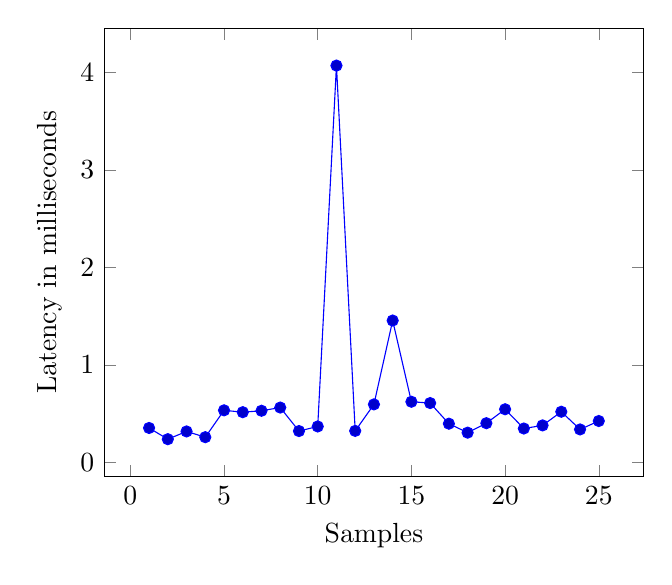
\begin{tikzpicture}
        \begin{axis}[
            xlabel=Samples,
            ylabel=Latency in milliseconds]
            \addplot coordinates {(1,0.352) (2,0.237) (3,0.3165) (4,0.2575) (5,0.533) (6,0.514) (7,0.5285) (8,0.5615) (9,0.3205) (10,0.3675) (11,4.069) (12,0.322) (13,0.594) (14,1.454) (15,0.621) (16,0.6075) (17,0.396) (18,0.304) (19,0.401) (20,0.544) (21,0.3465) (22,0.3785) (23,0.5185) (24,0.337) (25,0.4235) };
        \end{axis}
    \end{tikzpicture}
    \caption{Base-line Cisco Switch: Latency test (One way)}
    \label{CiscoLat}
\end{figure}


    \newpage
    % Here you present an interpretation of the results and assess their significance. Discuss the possible consequences of the results and present any recommendations. It is important that you report on whether you have achieved the goals you set and thus answered your research question and achieved the purpose/aim of the work. The section should also contain reflections on the work, such as its limitations. You can also discuss solutions to problems that you have identified and discussed previously or address other problems that the work has not addressed, questions that have not been answered. Also link your results to previous work. This way the discussion can become a conversation with what you wrote in previous sections. Finally, put your own work into a wider context, broaden your perspective. Can your results be generalized? Can what you have done be used in some other context?
\section{Discussion}
In this section you will talk about the results, was it expected, did something intresting happen and so on.

\subsection{Limitation}
    \newpage
    % In this section you will summarize the report and present conclusions and final analysis. Give a brief overview of the purpose and the question. You should then clearly talk about the most important results, explain their significance and put them into context. All conclusions should be supported in earlier parts of the report. However, you should not present new details.

% An expert should be able to read this section independently of the rest of the report.


\section{Conclusions}
This is your conclusions for the report, an \textit{important} part of this section is that \textbf{nothing new should be presented here}.
    \newpage
    % Here you will discuss what remains to be done. You can address improvements that can be made, and extensions of your work that can result in new issues for the future.

% If it is short, can be written in the "Conclusions" section.


\section{Future Work}
This section will present what can be elaborated on top of your work and what new paths opened up for future research.

% ==========

\glsresetall % resets all abbreviations for the reference

% ============================= References ============================
%\pagenumbering{roman}
% Comment out these lines if you don't need a list of references.
    %TC:ignore
    \clearpage
    \phantomsection
    \printbibliography[heading=bibintoc]
    %TC:endignore
% ============================= Appendices ============================
% Comment out these lines if you don't need a any appendices

\glsresetall % resets all abbreviations for the appendixes
    %TC:ignore
    \clearpage
    \begin{appendices}
       % Other information that does not fit directly into the text, but which may be of interest to a reader who wants to get in-depth, you place as attachments at the end of the report. It can be, for example, source code for an implementation, test data, images of a prototype etc.
\section{First appendix}\label{appen1}
some text for the appendix and a Table \ref{tab1}

\begin{table}
    \begin{tabular}{lll}
        \multicolumn{3}{c}{table}                                                \\
        1             & \multicolumn{1}{c}{\textit{2}} & \multicolumn{1}{r}{3}   \\
        \textbf{text} & \textbf{stuff}                 & \textbf{and more stuff}
    \end{tabular}
    \caption{a table}
    \label{tab1}
\end{table}

    \end{appendices}
     %TC:endignore
% ============================ Document End ===========================
\end{document}
